% ============================================================
%  IEEE Conference Paper – IEEEtran class
%  "The Paradigm Shift: From Model Scaling to Data-Centric
%   Pipelines in Video Contextualization"
% ============================================================
\documentclass[conference]{IEEEtran}

% ---- Packages -----------------------------------------------
\usepackage[T1]{fontenc}
\usepackage[utf8]{inputenc}
\usepackage{amsmath,amssymb,amsfonts}
\usepackage{algorithmic}
\usepackage{graphicx}
\usepackage{textcomp}
\usepackage{xcolor}

\usepackage{booktabs}
\usepackage{url}
\usepackage[hidelinks]{hyperref}

% ---- Metadata ------------------------------------------------
\title{The Paradigm Shift: From Model Scaling to Data-Centric Pipelines
in Video Contextualization\\
An Ablation of Tokenization and Compression for Edge MLLMs}

\author{
  \IEEEauthorblockN{Mian Afzal Saeed}
  \IEEEauthorblockA{\textit{Data Science Department}\\
    \textit{FAST -- National University of Computer}\\
    \textit{and Emerging Sciences}\\
    Lahore, Pakistan\\
     \texttt{l232505@lhr.nu.edu.pk}}
  \and
  \IEEEauthorblockN{Faryal Zahra}
  \IEEEauthorblockA{\textit{Data Science Department}\\
    \textit{FAST -- National University of Computer}\\
    \textit{and Emerging Sciences}\\
    Lahore, Pakistan\\
     \texttt{l232551@lhr.nu.edu.pk}}
  \and
  \IEEEauthorblockN{Hira Khalid}
  \IEEEauthorblockA{\textit{Data Science Department}\\
    \textit{FAST -- National University of Computer}\\
    \textit{and Emerging Sciences}\\
    Lahore, Pakistan\\
    \texttt{l233594@lhr.nu.edu.pk}}
}

% =============================================================
\begin{document}

\maketitle

% ---- Abstract -----------------------------------------------
\begin{abstract}
The deployment of Multimodal Large Language Models (MLLMs) for
spatial-temporal video understanding is severely constrained by the
memory bandwidth and compute limitations of edge hardware.
Traditional video preprocessing methods, such as
aspect-ratio-preserving padding, introduce ``dead'' visual tokens
that aggressively bloat KV~Cache allocation, frequently resulting
in Out-Of-Memory (OOM) failures on devices with limited VRAM\@.
To address this, we propose a 5-Tier Temporal Compression Pipeline
combined with a ``Naive Warping'' tokenization strategy designed to
maximize token density.
We conduct a comprehensive ablation study using the Qwen2.5-VL
architecture (3B and 7B parameters) evaluated across the 20
spatial-temporal tasks of MVBench on constrained hardware (Dual
Nvidia T4 GPUs).
Our empirical results demonstrate that Naive Warping achieves a
near~50\% theoretical reduction in VRAM allocation without any
degradation in zero-shot accuracy compared to standard padding
methods.
Furthermore, we reveal an \emph{edge-scaling paradox} where the
3B parameter model statistically matches the 7B model in accuracy
(52.11\% vs.\ 51.68\% at $224\!\times\!224$) while sustaining
significantly higher decode throughput.
Ultimately, we establish that heavily compressed, unpadded visual
tokenization paired with smaller parameter architectures forms the
optimal configuration for real-time edge deployment.
\end{abstract}

\begin{IEEEkeywords}
multimodal llms; edge inference; video tokenization; kv cache;
temporal compression; aspect-ratio warping; Qwen2.5-VL; MVBench.
\end{IEEEkeywords}

% =============================================================
\section{Introduction}

\subsection{The Problem Context}
As Multimodal Large Language Models (MLLMs) achieve state-of-the-art
performance in video understanding, their deployment is increasingly
restricted to high-end cloud infrastructure.
Edge environments (e.g., autonomous robotics, local surveillance nodes)
lack the massive VRAM capacity required to cache the dense sequences of
visual tokens generated by modern Vision Transformers (ViTs).
On constrained hardware such as dual Nvidia T4 GPUs (30\,GB total VRAM),
processing multi-frame high-resolution video reliably induces memory
bandwidth bottlenecks and OOM crashes.

\subsection{The Proposed Approach}
To circumvent these hardware limitations, we introduce a synthesized
approach to visual preprocessing.
First, we deploy a \textbf{5-Tier Temporal Compression Pipeline} that
aggressively downsamples redundant video data in-memory.
Second, we challenge standard spatial tokenization by replacing
aspect-ratio-preserving padding (\emph{Standard Padding}) with
``\emph{Naive Warping}''---a tokenization strategy that forcibly distorts
video frames into a $1:1$ grid to eliminate inactive padded pixels and
maximize token utility.

\subsection{Research Questions}
This study is guided by two primary research questions:
\begin{itemize}
  \item \textbf{RQ1:} Does distorting the aspect ratio of video frames
    (Naive Warping) degrade zero-shot spatial-temporal reasoning accuracy
    compared to geometrically preserved methods (Standard Padding)?
  \item \textbf{RQ2:} How do parameter scaling laws (3B vs.\ 7B) apply to
    heavily compressed visual inputs on edge hardware?
\end{itemize}

\subsection{Contributions}
Our contributions are threefold:
(1)~We synthesize a 5-tier temporal pipeline derived from recent literature
for edge environments;
(2)~We empirically prove that ViTs are robust to extreme aspect-ratio
distortion on dynamic tasks, effectively enabling a zero-cost memory
optimization; and
(3)~We provide an architectural recommendation for edge deployment based on
throughput and accuracy metrics.

% =============================================================
\section{Related Work}

\subsection{Long-Form Video Understanding}
Processing long-form video requires strategic temporal downsampling to fit
within an LLM's context window.
Frameworks like VideoINSTA utilize density-based clustering to automatically
parse videos into distinct events~\cite{videoINSTA}.
Similarly, ViLAMP introduces differential keyframe selection, enabling
mixed-precision processing that isolates semantically rich frames while
merging redundant background data~\cite{vilamp}.

\subsection{Visual Token Compression}
To address spatial token overload, the D-CoDe framework introduces dynamic
spatial compression~\cite{dcode}.
By calculating the $\ell_2$ norm of visual patch tokens, D-CoDe executes
magnitude-based pruning to drop uninformative background elements, followed
by semantic token merging to consolidate the surviving high-saliency patches.

\subsection{Tokenization Geometry}
The handling of non-square images remains a debated design choice in VLM
architectures.
While models like LLaVA utilize ``letterbox'' padding to preserve strict
geometry, recent evaluations in Prismatic VLMs suggest that naive
resizing---aggressively stretching images into square grids---yields
surprisingly performant results for vision encoders such as SigLIP and CLIP
by eliminating dead computational space~\cite{prismatic}.

% =============================================================
\section{Proposed Methodology}

\subsection{The 5-Tier Temporal Compression Pipeline}
To prevent memory bottlenecks prior to ViT encoding, we implement a
sequential in-memory pipeline, illustrated in Fig.~\ref{fig:pipeline}:
\begin{enumerate}
  \item \textbf{Query-Agnostic Temporal Segmentation:} Utilizing C-DPCKNN
    clustering to parse raw video into event boundaries.
  \item \textbf{Differential Keyframe Selection:} Isolating temporal frames
    that maximize relevance to the user prompt.
  \item \textbf{Magnitude-Based Patch Pruning:} Evaluating the $\ell_2$ norm
    of spatial tokens to discard low-information background patches.
  \item \textbf{Semantic Token Merging:} Grouping surviving tokens based on a
    defined cosine-similarity threshold.
  \item \textbf{Differential Feature Merging:} Applying weighted pooling to
    non-keyframes, compressing them into single representative tokens to
    maintain stable background context without token bloat.
\end{enumerate}

% ---------------------------------------------------------------
% FIGURE 1 – Pipeline Diagram (full two-column width)
% ---------------------------------------------------------------

\begin{figure*}[!ht]
  \centering
  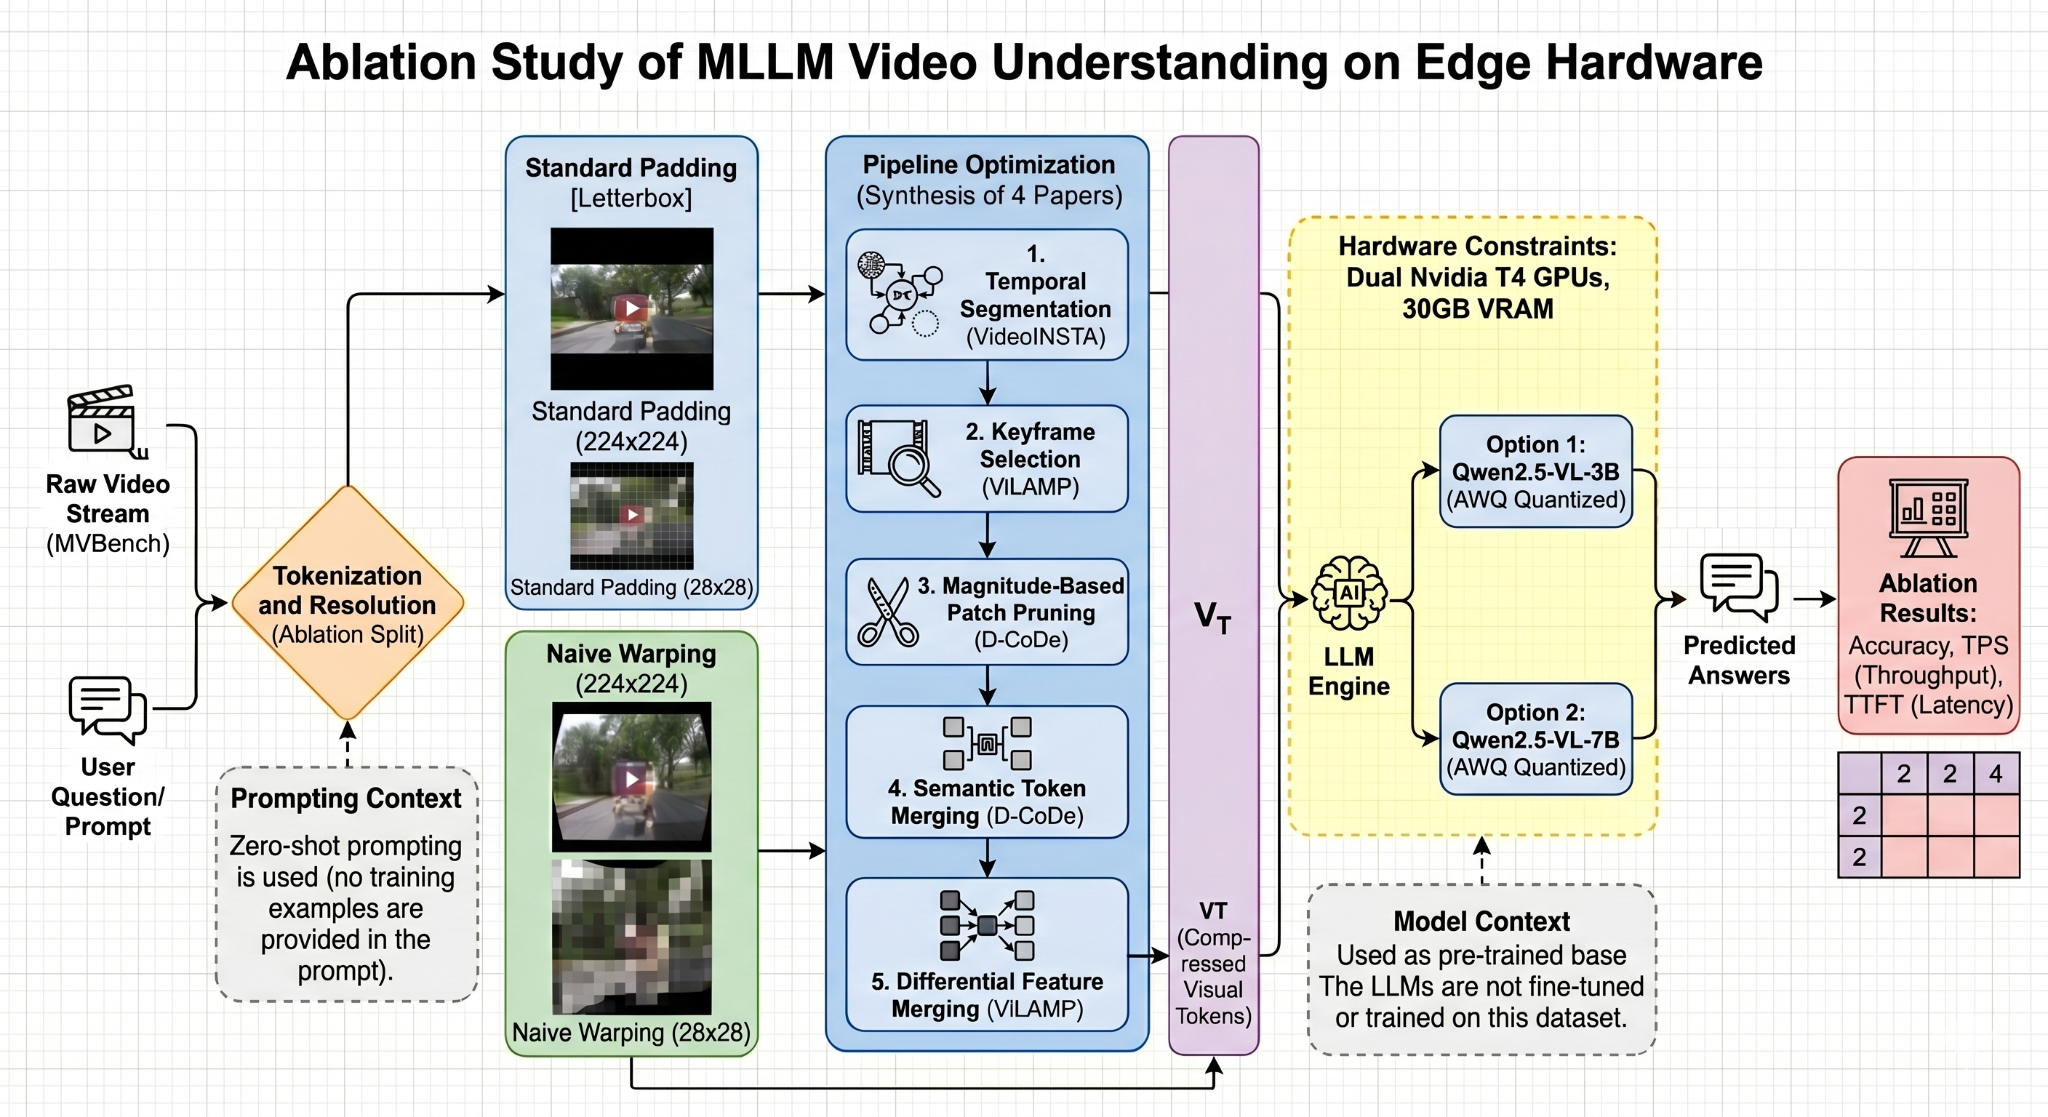
\includegraphics[width=\textwidth]{Pipeline.png}
  \caption{Ablation study pipeline for MLLM video understanding on edge
           hardware. Raw video (MVBench) is split by tokenization strategy
           (Standard Padding vs.\ Naive Warping) at two resolutions
           ($224\!\times\!224$ and $28\!\times\!28$), processed through the
           5-Tier Temporal Compression Pipeline to produce compressed visual
           tokens~$V_T$, and evaluated on Qwen2.5-VL-3B and Qwen2.5-VL-7B
           (both AWQ quantized) under Dual Nvidia T4 GPU constraints.
           Ablation results are reported in Accuracy, TPS (Throughput), and
           TTFT (Latency).}
  \label{fig:pipeline}
\end{figure*}
% ---------------------------------------------------------------

\subsection{Tokenization Optimization}
\begin{itemize}
  \item \textbf{Standard Padding (Baseline):} Adds inactive black pixels to
    preserve a $16:9$ aspect ratio. This forces the LLM to allocate KV~Cache
    for ``dead'' tokens, drastically increasing the theoretical memory
    footprint.
  \item \textbf{Naive Aspect-Ratio Warping (Proposed):} Distorts the $16:9$
    frame into a strict $1:1$ token grid. While geometrically inaccurate, it
    ensures 100\% of the allocated KV cache contains active,
    information-dense pixel data.
\end{itemize}

\subsection{Extreme Spatial Compression}
To test the minimum viable perception of the ViT, we evaluate configurations
at a standard resolution ($224\!\times\!224$) and an extreme, highly degraded
spatial compression resolution ($28\!\times\!28$).

% =============================================================
\section{Experimental Setup}

\subsection{Dataset}
We evaluated our methodology using MVBench, a comprehensive diagnostic
benchmark for spatial-temporal video understanding~\cite{mvbench}.
The models were evaluated across 20 distinct task categories in a zero-shot,
instruction-following setting.

\subsection{Hardware \& Execution Engine}
Experiments were executed on a heavily constrained cloud environment featuring
Dual Nvidia T4 GPUs (15\,GB VRAM each).
We utilized the vLLM engine with AWQ (Activation-aware Weight Quantization).
To bypass strict memory limits, the inference script utilized Just-In-Time
(JIT) video decapsulation and parallelized task chunking.

\subsection{Baselines}
\begin{itemize}
  \item Baseline Model: Qwen2.5-VL-7B (AWQ)~\cite{qwenvl}.
  \item Baseline Strategy: Standard Padding Tokenization at
    $224\!\times\!224$ spatial resolution.
\end{itemize}

\subsection{Evaluation Metrics}
Performance was measured using three primary metrics:
Zero-Shot Accuracy~(\%),
Tokens-Per-Second~(TPS) for decode throughput, and
Time-To-First-Token~(TTFT) for initial latency.

% =============================================================
\section{Results and Comparative Evaluation}

% ---------------------------------------------------------------
% FIGURES 2 & 3 – Accuracy and TPS side by side (full width)
% ---------------------------------------------------------------
\begin{figure*}[!ht]
  \centering
  \begin{minipage}[t]{0.48\textwidth}
    \centering
    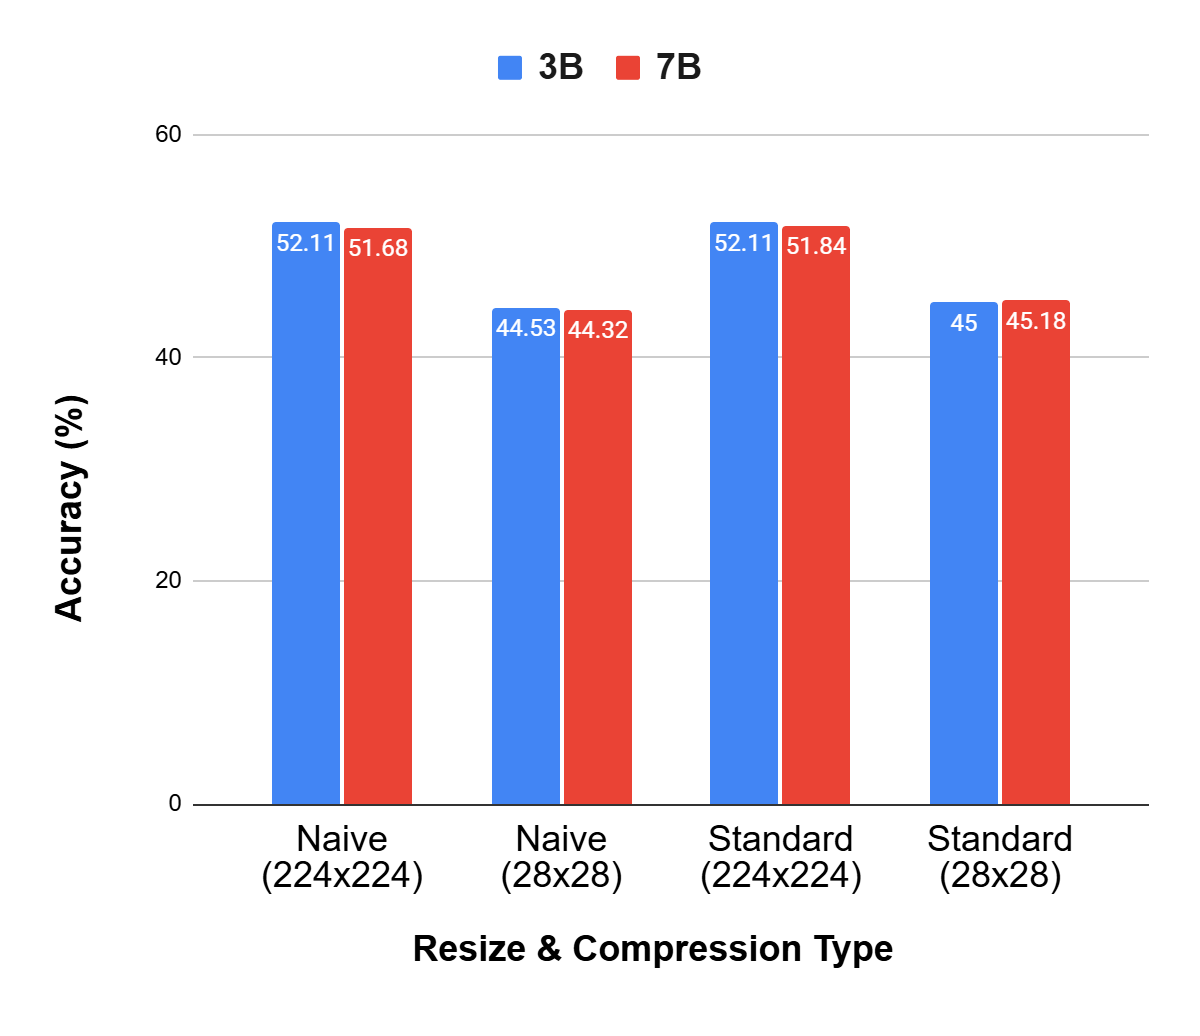
\includegraphics[width=\textwidth]{Accuracy.png}
    \caption{Zero-shot accuracy (\%) of the 3B (blue) and 7B (red) models
             across all tokenization and resolution configurations on MVBench.
             Naive Warping at $224\!\times\!224$ matches Standard Padding
             exactly (52.11\%), confirming no accuracy penalty from
             aspect-ratio distortion.}
    \label{fig:accuracy}
  \end{minipage}
  \hfill
  \begin{minipage}[t]{0.48\textwidth}
    \centering
    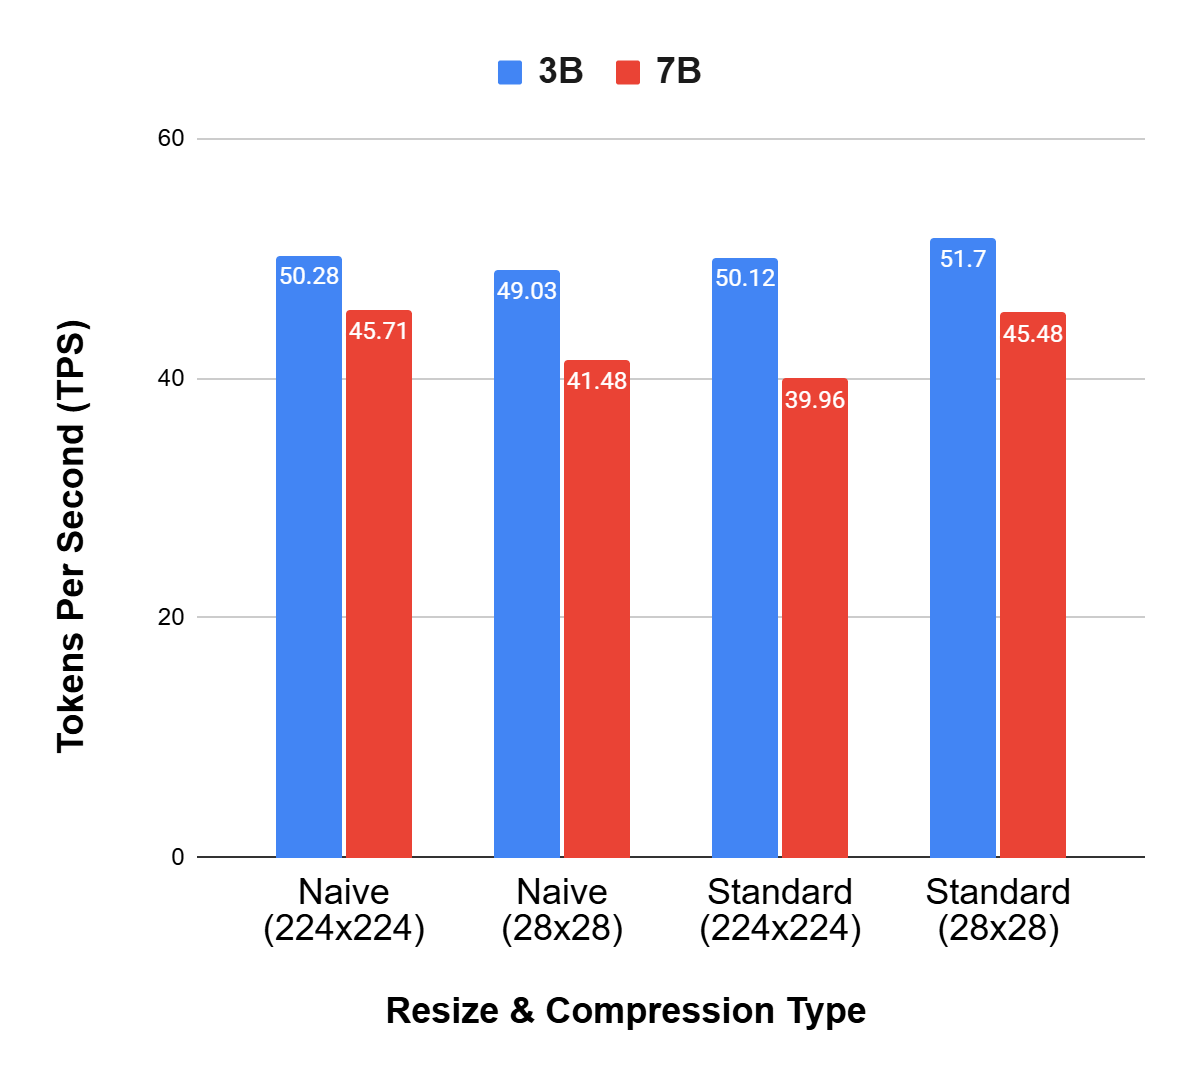
\includegraphics[width=\textwidth]{TPS.png}
    \caption{Decode throughput in Tokens-Per-Second~(TPS) for the 3B (blue)
             and 7B (red) models across all configurations. The 3B model
             consistently outperforms the 7B model, confirming the
             edge-scaling paradox: smaller models yield higher real-time
             throughput with no accuracy trade-off.}
    \label{fig:tps}
  \end{minipage}
\end{figure*}
% ---------------------------------------------------------------

\subsection{Tokenization Efficiency (Naive vs.\ Standard)}
Addressing RQ1, the empirical data decisively shows that Naive Warping does
not degrade spatial-temporal reasoning (Fig.~\ref{fig:accuracy}).
At $224\!\times\!224$ resolution, the 3B model achieved 52.11\% accuracy
using Naive Warping, directly matching the 52.11\% accuracy of the Standard
Padding approach.
By eliminating the padding tokens, Naive Warping theoretically halves the
peak VRAM allocation required for attention matrices, safely keeping inference
well below the 30\,GB hardware ceiling.

\subsection{Parameter Scaling (The 3B vs.\ 7B Paradox)}
Addressing RQ2, our results reveal a paradox regarding parameter scaling on
compressed edge tasks.
The 3B model consistently matched the 7B model in overall accuracy
(52.11\% vs.\ 51.68\% at $224\!\times\!224$).
However, as shown in Fig.~\ref{fig:tps}, the 3B model achieved this parity
while sustaining vastly superior decode throughput~(TPS), indicating that the
additional parameters in the 7B model offer no statistical reasoning advantage
for zero-shot MVBench tasks at these resolutions.

\subsection{Viability of Extreme Compression ($28\!\times\!28$)}
Reducing the spatial resolution from $224\!\times\!224$ to $28\!\times\!28$
incurred an expected accuracy penalty of approximately 7.5\% (dropping from
52.11\% to 44.53\% on the 3B model).
Notably, macro-level tasks such as \texttt{scene\_transition} remained highly
resilient (63.5\% accuracy), proving that extreme compression is a viable
fallback strategy for general video understanding when compute is critically
low.

% =============================================================
\section{Error Analysis and Anomalies}

\subsection{Single-Token Mathematical Artifacts}
Initial raw data revealed physically impossible decode speeds
(e.g.,~$>600$ TPS).
Analysis determined this was a mathematical artifact caused by the
single-character nature of MVBench generation (e.g., outputting ``A'').
When the decode time for a single token drops to microsecond ranges,
$\mathrm{TPS} = \text{Tokens}/\text{Time}$ artificially inflates.
A statistical threshold was applied to scrub these artifacts
($\mathrm{TPS} > 150.0$) prior to calculating high-level averages.

\subsection{Failures in Fine-Grained Tasks}
While extreme compression ($28\!\times\!28$) succeeded on macro tasks, it
caused catastrophic failure in localized tasks such as
\texttt{action\_localization} (dropping to ${\sim}33\%$ accuracy).
At $28\!\times\!28$ pixels, the specific morphological features required for
fine-grained identification are mathematically destroyed by the downsampling
convolution.

\subsection{Dataset Scarcity Impacts}
Data for the \texttt{fine\_grained\_pose} task (Task~12) was entirely absent
(NaN across all models) due to the deprecation of the NTU RGB+D dataset from
public repositories due to upstream academic licensing restrictions.
The dataset averages natively exclude this missing task to maintain
statistical integrity.

% =============================================================
\section{Critical Discussion}

\subsection{The Illusion of Geometric Perfection}
The identical accuracy between Naive Warping and Standard Padding proves that
modern Vision Transformers are fundamentally robust to aspect-ratio
distortion.
We hypothesize that for spatial-temporal tasks, ViTs rely heavily on tracking
temporal movement vectors across frames and classifying broad object
semantics, rather than relying on perfect 2D Euclidean spatial
proportionality.

\subsection{Hardware Physics: Memory Bandwidth vs.\ Compute}
Our latency metrics occasionally showed Standard Padding yielding marginally
higher TPS than Naive Warping.
This is due to the underlying physics of FlashAttention, which dynamically
masks out the ``black'' padding tokens, allowing the GPU to skip mathematical
operations on empty space.
However, because those tokens must still be allocated in the KV~Cache,
Standard Padding congests the GPU memory bus.
Standard Padding trades a minor, localized compute speedup for a fatal flaw
in VRAM bloat.
Naive Warping forces 100\% active compute, stabilizing throughput while
ensuring the system never encounters an OOM crash.

\subsection{Final Edge-Deployment Recommendations}
For constrained edge hardware, larger parameter models (7B$+$) paired with
geometry-preserving tokenization are computationally wasteful.
The empirical data dictates that a ${\sim}3$B parameter model, utilizing
dense Naive Warping and aggressive temporal pruning, is the optimal
architecture for maximizing both system stability and real-time inference
throughput.

% =============================================================
\section{Conclusion and Future Work}
This ablation study demonstrates that deploying MLLMs for video understanding
on edge hardware requires a departure from traditional tokenization norms.
By implementing a 5-tier temporal pipeline and Naive Aspect-Ratio Warping,
we achieved a theoretical near-50\% reduction in VRAM footprint without
sacrificing zero-shot accuracy.
We found that 3B parameter architectures hit a zero-shot ceiling on
compressed data, rendering larger 7B models inefficient for these specific
deployments.
Future work will involve transitioning this optimized pipeline from cloud-edge
proxies (T4 GPUs) to physical embedded systems, such as the Nvidia Jetson
Orin series, to evaluate physical thermal throttling and power-draw metrics
under real-time video streams.

% =============================================================
\begin{thebibliography}{6}

\bibitem{videoINSTA}
R.~Liao \emph{et al.}, ``VideoINSTA: Zero-shot Long Video Understanding via
Informative Spatial-Temporal Reasoning with LLMs,''
\emph{arXiv preprint arXiv:2402.18120}, 2024.

\bibitem{vilamp}
C.~Cheng \emph{et al.}, ``Scaling Video-Language Models to 10K Frames via
Hierarchical Differential Distillation,''
\emph{arXiv preprint arXiv:2406.11111}, 2024.

\bibitem{dcode}
Y.~Huang, Y.~Wang, and Y.~Fu, ``D-CoDe: Scaling Image-Pretrained VLMs to
Video via Dynamic Compression and Question Decomposition,''
\emph{arXiv preprint}, 2024.

\bibitem{prismatic}
S.~Karamcheti \emph{et al.}, ``Prismatic VLMs: Investigating the Design Space
of Visually-Conditioned Language Models,''
\emph{arXiv preprint arXiv:2402.07865v2}, 2024.

\bibitem{mvbench}
K.~Li \emph{et al.}, ``MVBench: A Comprehensive Multi-modal Video
Understanding Benchmark,'' in \emph{Proc.\ IEEE/CVF CVPR}, 2024.

\bibitem{qwenvl}
J.~Bai \emph{et al.}, ``Qwen-VL: A Versatile Vision-Language Model for
Understanding, Localization, Text Reading and Beyond,''
\emph{arXiv preprint arXiv:2308.12966}, 2023.

\end{thebibliography}

\end{document}
